\documentclass{article}

\usepackage{tikz} 
% Added arrows.meta for cleaner arrowheads
\usetikzlibrary{automata, positioning, arrows, arrows.meta} 

\usepackage{amsthm}
\usepackage{amsfonts}
\usepackage{amsmath}
\usepackage{amssymb}
\usepackage{fullpage}
\usepackage{color}
\usepackage{parskip}
\usepackage{hyperref}
  \hypersetup{
    colorlinks = true,
    urlcolor = blue,       % color of external links using \href
    linkcolor= blue,       % color of internal links 
    citecolor= blue,       % color of links to bibliography
    filecolor= blue,        % color of file links
    }
    
\usepackage{listings}
\usepackage[utf8]{inputenc}                                                    
\usepackage[T1]{fontenc}                                                       
\usepackage{booktabs}
\usepackage{forest}

\definecolor{dkgreen}{rgb}{0,0.6,0}
\definecolor{gray}{rgb}{0.5,0.5,0.5}
\definecolor{mauve}{rgb}{0.58,0,0.82}

\lstset{frame=tb,
  language=haskell,
  aboveskip=3mm,
  belowskip=3mm,
  showstringspaces=false,
  columns=flexible,
  basicstyle={\small\ttfamily},
  numbers=none,
  numberstyle=\tiny\color{gray},
  keywordstyle=\color{blue},
  commentstyle=\color{dkgreen},
  stringstyle=\color{mauve},
  breaklines=true,
  breakatwhitespace=true,
  tabsize=3
}

\newtheoremstyle{theorem}
  {\topsep}   % ABOVESPACE
  {\topsep}   % BELOWSPACE
  {\itshape\/}  % BODYFONT
  {0pt}       % INDENT (empty value is the same as 0pt)
  {\bfseries} % HEADFONT
  {.}         % HEADPUNCT
  {5pt plus 1pt minus 1pt} % HEADSPACE
  {}          % CUSTOM-HEAD-SPEC
\theoremstyle{theorem} 
   \newtheorem{theorem}{Theorem}[section]
   \newtheorem{corollary}[theorem]{Corollary}
   \newtheorem{lemma}[theorem]{Lemma}
   \newtheorem{proposition}[theorem]{Proposition}
\theoremstyle{definition}
   \newtheorem{definition}[theorem]{Definition}
   \newtheorem{example}[theorem]{Example}
\theoremstyle{remark}    
  \newtheorem{remark}[theorem]{Remark}

% ==========================================
% Global TikZ Settings for Automata Diagrams
% ==========================================
\tikzset{
    ->, % Directed edges
    >=stealth, % Nice arrowheads
    node distance=3cm, % Standard distance between nodes
    every state/.style={thick, fill=gray!10}, % Styling for states
    initial text=$ $, % Removes the "start" text on the initial arrow
}

\title{CPSC-406 Report}
\author{Farzana Chowdhury  \\ Chapman University}

\date{\today} 

\begin{document}

\maketitle

\begin{abstract}
\end{abstract}

\setcounter{tocdepth}{3}
\tableofcontents
\newpage

\section{Introduction}\label{intro}

\section{Week by Week}\label{homework}

\subsection{Week 1}

\subsubsection{DFAs}

\textbf{Exercise 1}

\textbf{1. Which of the following words are accepted/refused by $\mathcal{A}_1$ and $\mathcal{A}_2$? Complete the table.}

\begin{center}
\renewcommand{\arraystretch}{1.5}
\begin{tabular}{|c|c|c|}
\hline
\textbf:{$w$} & \textbf{accepted by $\mathcal{A}_1$?} & \textbf{accepted by $\mathcal{A}_2$?} \\
\hline
$aaa$ & $\times$ & \checkmark \\
\hline
$aab$ & \checkmark & $\times$ \\
\hline
$aba$ & $\times$ & $\times$ \\
\hline
$abb$ & $\times$ & $\times$ \\
\hline
$baa$ & $\times$ & \checkmark \\
\hline
$bab$ & $\times$ & $\times$ \\
\hline
$bba$ & $\times$ & $\times$ \\
\hline
$bbb$ & $\times$ & $\times$ \\
\hline
\end{tabular}
\end{center}

\vspace{0.5cm}
\textbf{2. More generally, can you completely describe the languages $L(\mathcal{A}_k)$ accepted by $\mathcal{A}_k$, for $k=1, 2$?}

\begin{itemize}
	\item $L(\mathcal{A}_1)$: The language of all words over $\{a, b\}$ that start with the letter $a$ and end with an odd number of consecutive $b$'s. 
        
    \item $L(\mathcal{A}_2)$: The language of all words over $\{a, b\}$ that end with the substring $aa$. 
    
\end{itemize}

\vspace{0.5cm}

\textbf{Exercise 2}

\textbf{Design DFAs whose accepted languages are given as follows:}

% ---------------------------------------------------------
\vspace{0.5cm}
\textbf{1. All the words that end with $ab$}

\begin{center}
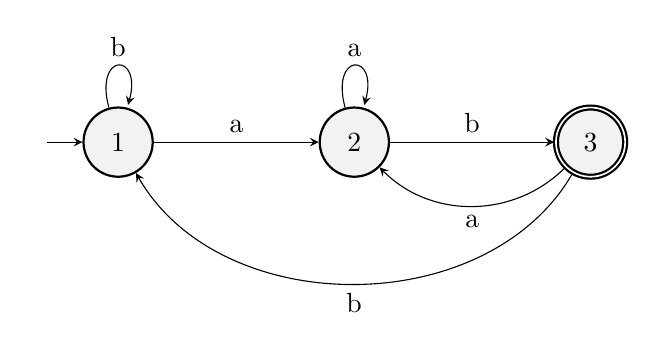
\begin{tikzpicture}
    \node[state, initial] (q1) {1};
    \node[state] (q2) [right of=q1] {2};
    \node[state, accepting] (q3) [right of=q2] {3};

    \path
        (q1) edge [loop above] node {b} (q1)
             edge node[above] {a} (q2)
        (q2) edge [loop above] node {a} (q2)
             edge node[above] {b} (q3)
        (q3) edge [bend left=45] node[below] {a} (q2)
             edge [bend left=60] node[below] {b} (q1);
\end{tikzpicture}
\end{center}

% ---------------------------------------------------------
\vspace{0.5cm}
\textbf{2. All the words that contain $aba$}

\begin{center}
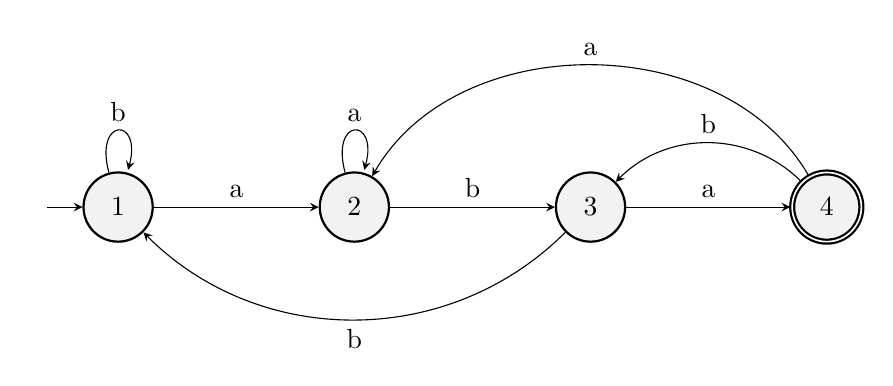
\begin{tikzpicture}
    \node[state, initial] (q1) {1};
    \node[state] (q2) [right of=q1] {2};
    \node[state] (q3) [right of=q2] {3};
    \node[state, accepting] (q4) [right of=q3] {4};

    \path
        (q1) edge [loop above] node {b} (q1)
             edge node[above] {a} (q2)
        (q2) edge [loop above] node {a} (q2)
             edge node[above] {b} (q3)
        (q3) edge [bend left=45] node[below] {b} (q1)
             edge node[above] {a} (q4)
        (q4) edge [bend right=60] node[above] {a} (q2)
             edge [bend right=45] node[above] {b} (q3);
\end{tikzpicture}
\end{center}

% ---------------------------------------------------------
\vspace{0.5cm}
\textbf{3. All the words that contain an odd number of $a$'s and an odd number of $b$'s}

\begin{center}
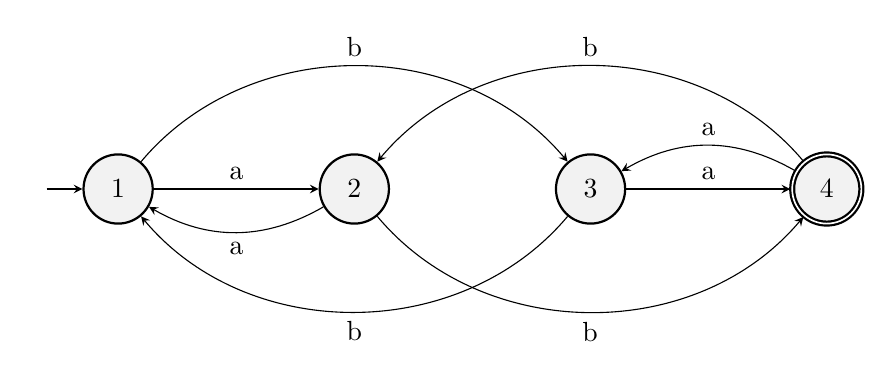
\begin{tikzpicture}
    \node[state, initial] (q1) {1};
    \node[state] (q2) [right of=q1] {2};
    \node[state] (q3) [right of=q2] {3};
    \node[state, accepting] (q4) [right of=q3] {4};

    \path
        (q1) edge node[above] {a} (q2)
             edge [bend left=50] node[above] {b} (q3)
        (q2) edge [bend left] node[below] {a} (q1)
             edge [bend right=50] node[below] {b} (q4)
        (q3) edge [bend left=50] node[below] {b} (q1)
             edge node[above] {a} (q4)
        (q4) edge [bend right=50] node[above] {b} (q2)
             edge [bend right] node[above] {a} (q3);
\end{tikzpicture}
\end{center}

% ---------------------------------------------------------
\vspace{0.5cm}
\textbf{4. All the words that contain an even number of $a$'s and an odd number of $b$'s}

\begin{center}
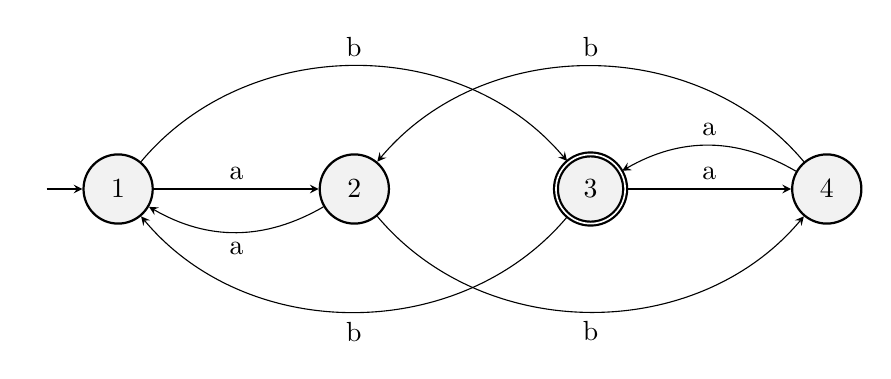
\begin{tikzpicture}
    \node[state, initial] (q1) {1};
    \node[state] (q2) [right of=q1] {2};
    \node[state, accepting] (q3) [right of=q2] {3};
    \node[state] (q4) [right of=q3] {4};

    \path
        (q1) edge node[above] {a} (q2)
             edge [bend left=50] node[above] {b} (q3)
        (q2) edge [bend left] node[below] {a} (q1)
             edge [bend right=50] node[below] {b} (q4)
        (q3) edge [bend left=50] node[below] {b} (q1)
             edge node[above] {a} (q4)
        (q4) edge [bend right=50] node[above] {b} (q2)
             edge [bend right] node[above] {a} (q3);
\end{tikzpicture}
\end{center}

% ---------------------------------------------------------
\vspace{0.5cm}
\textbf{5. All the words such that any three consecutive characters contain at least one $a$}

\begin{center}
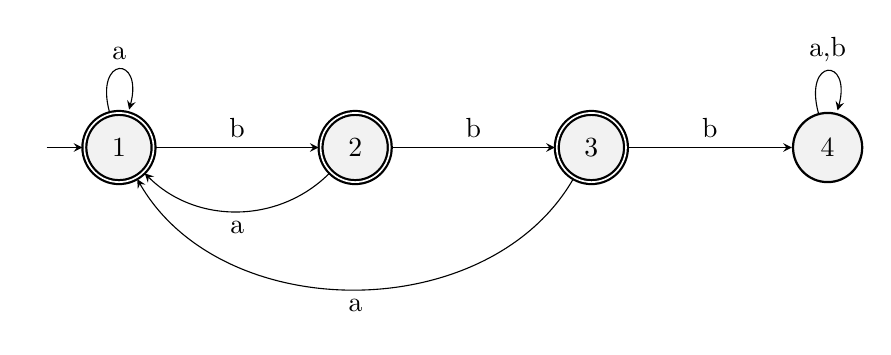
\begin{tikzpicture}
    \node[state, initial, accepting] (q1) {1};
    \node[state, accepting] (q2) [right of=q1] {2};
    \node[state, accepting] (q3) [right of=q2] {3};
    \node[state] (q4) [right of=q3] {4};

    \path
        (q1) edge [loop above] node {a} (q1)
             edge node[above] {b} (q2)
        (q2) edge [bend left=45] node[below] {a} (q1)
             edge node[above] {b} (q3)
        (q3) edge [bend left=60] node[below] {a} (q1)
             edge node[above] {b} (q4)
        (q4) edge [loop above] node {a,b} (q4);
\end{tikzpicture}
\end{center}

% ---------------------------------------------------------
\vspace{0.5cm}
\textbf{6. All the words that contain $bbb$}

\begin{center}
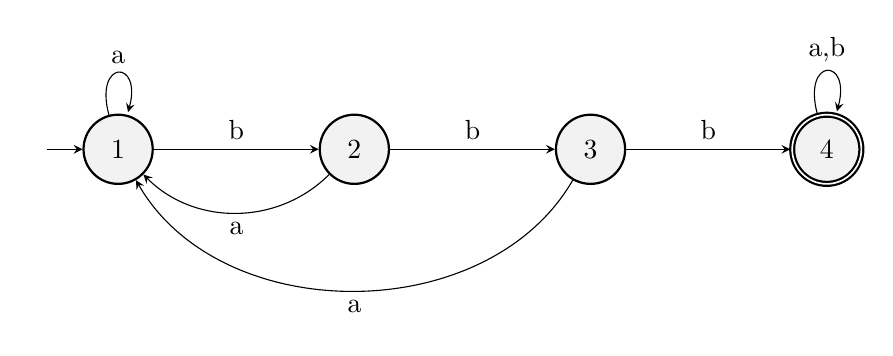
\begin{tikzpicture}
    \node[state, initial] (q1) {1};
    \node[state] (q2) [right of=q1] {2};
    \node[state] (q3) [right of=q2] {3};
    \node[state, accepting] (q4) [right of=q3] {4};

    \path
        (q1) edge [loop above] node {a} (q1)
             edge node[above] {b} (q2)
        (q2) edge [bend left=45] node[below] {a} (q1)
             edge node[above] {b} (q3)
        (q3) edge [bend left=60] node[below] {a} (q1)
             edge node[above] {b} (q4)
        (q4) edge [loop above] node {a,b} (q4);
\end{tikzpicture}
\end{center}

\textbf{What do you notice when comparing the various automata?}

For DFAs that have criteria of "ends with," arrows must leave the accept state because the string could keep going and fail to satisfy DFA characteristics. For DFAs that have criteria of "contains," the accept state must be a "Trap State" with a self-loop, because once you find the sequence, you can traverse through the DFA while satisfying DFA's accepted language conditions.

\subsubsection{Question}
What is the easiest and best way to implement DFAs in programming?

\subsection{Week 2}

\subsubsection{Operations on automata}

\textbf{Exercise 1}
\begin{enumerate}
  \item $L(\mathcal{A}^{(1)})$ can't have $aa$ or $bb$ (two of the same letters in a row). For $L(\mathcal{A}^{(1)})$, any $a$ has to be in an odd numbered state position.
  \item
  \begin{center}
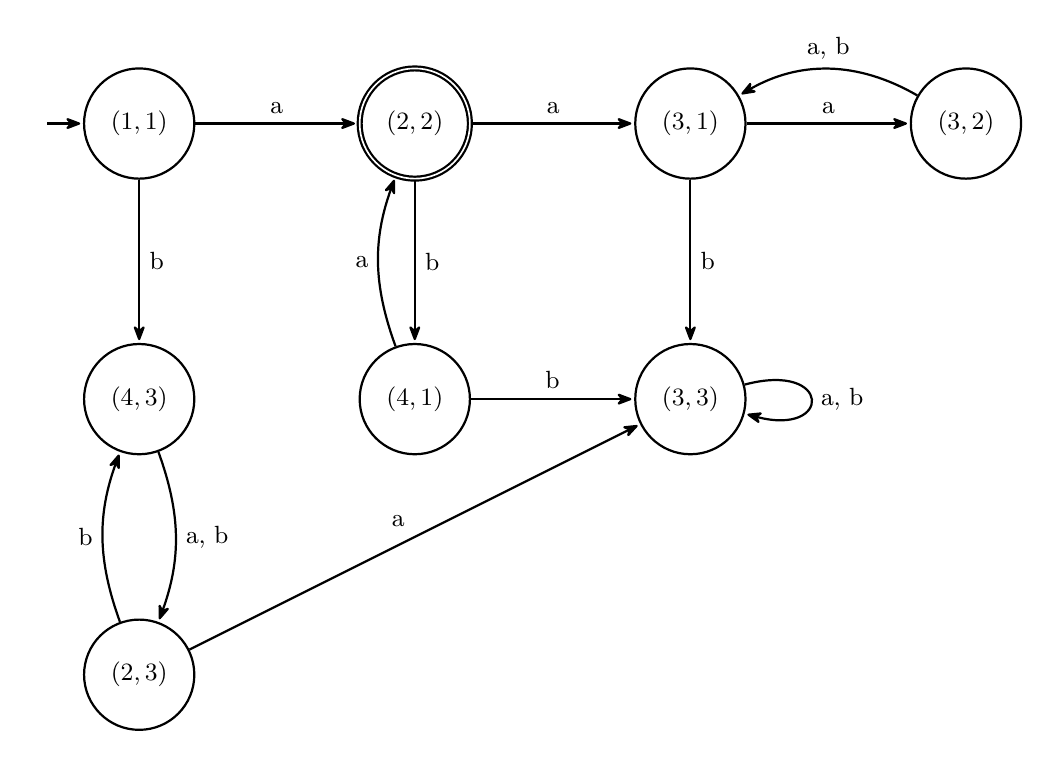
\begin{tikzpicture}[
    shorten >=1pt, node distance=3.5cm, on grid, auto, 
    thick, initial text={}, 
    every state/.style={minimum size=1.4cm, font=\small},
    >={Stealth[round]},
    every node/.style={font=\small}
]

    % --- States ---
    \node[state, initial] (s11) {$(1,1)$};
    \node[state, accepting] (s22) [right=of s11] {$(2,2)$};
    \node[state] (s31) [right=of s22] {$(3,1)$};
    \node[state] (s32) [right=of s31] {$(3,2)$};
    
    \node[state] (s43) [below=of s11] {$(4,3)$};
    \node[state] (s41) [below=of s22] {$(4,1)$};
    \node[state] (s33) [below=of s31] {$(3,3)$};
    
    \node[state] (s23) [below=of s43] {$(2,3)$};

    % --- Transitions ---
    \path[->] 
        % Row 1
        (s11) edge node {a} (s22)          % Removed extra a
              edge node {b} (s43)
        
        (s22) edge node {a} (s31)          % Removed extra a
              edge node {b} (s41)
              
        (s31) edge node {a} (s32)
              edge node {b} (s33)
        
        (s32) edge [bend right=30] node[above] {a, b} (s31)
        
        % Row 2
        (s41) edge [bend left=20] node {a} (s22)
              edge node {b} (s33)          % Removed extra a
              
        (s43) edge [bend left=20] node {a, b} (s23)
        
        (s33) edge [loop right] node {a, b} (s33)
        
        % Row 3
        (s23) edge [bend left=20] node {b} (s43)
              edge node {a} (s33);         % Removed extra a

\end{tikzpicture}
\end{center}
  \item To find the intersection of two languages ($L_1 \cap L_2$), you create a new machine that simulates how $\mathcal{A}^{(1)}$ and $\mathcal{A}^{(2)}$ work at the same time. When you take in an input $a$ or $b$, both numbers in the pair update at the same time based on their original rules. For intersection ($\cap$), you only have a double circle if both machines are in an accepting state.
  \item For union ($\cup$), you have a double circle if at least one of the machines is in an accepting state.
\end{enumerate}   

\textbf{Exercise 2}
\begin{enumerate}
    \item For $L(\mathcal{B}^{(1)})$, the total number of $a$ is a multiple of 3, including zero. For $L(\mathcal{B}^{(2)})$, every $a$ is directly followed by at least one $b$, and the string must not end with $a$. 
    \item 
    %\begin{center}
\begin{tikzpicture}[
    shorten >=1pt, 
    node distance=2.4cm, % Optimized for standard page width
    on grid, 
    auto, 
    thick, 
    initial text={}, 
    every state/.style={minimum size=1.1cm, font=\scriptsize},
    >={Stealth[round]},
    every node/.style={font=\scriptsize}
]

    % --- States ---
    \node[state, initial, accepting] (p0q0) {$(p_0, q_0)$};
    \node[state] (p1q1) [right=of p0q0] {$(p_1, q_1)$};
    \node[state] (p1q0) [right=of p1q1] {$(p_1, q_0)$};
    
    \node[state] (p0q2) [below=of p0q0] {$(p_0, q_2)$};
    \node[state] (p2q2) [below=of p1q1] {$(p_2, q_2)$};
    \node[state] (p2q1) [below=of p1q0] {$(p_2, q_1)$};
    
    \node[state] (p1q2) [below=of p0q2] {$(p_1, q_2)$};
    \node[state] (p2q0) [below=of p2q1] {$(p_2, q_0)$};
    
    \node[state] (p0q1) [below=of p2q0] {$(p_0, q_1)$};

    % --- Transitions ---
    \path[->] 
        % Row 1
        (p0q0) edge [loop above] node {b} (p0q0)
               edge node {a} (p1q1)
               edge node[left] {a} (p0q2)
        (p1q1) edge node {b} (p1q0)
               edge node[left] {a} (p2q2)
        (p1q0) edge [loop above] node {b} (p1q0)
               edge node {a} (p2q1)
        
        % Row 2
        (p0q2) edge [loop left] node {b} (p0q2)
               edge node[swap] {a} (p1q2) 
        (p2q2) edge [loop right] node {b} (p2q2)
               edge [bend left=15] node {a} (p0q2)
        
        % RE-ROUTED: p2q1 to p0q2 (Underneath Row 2)
        % This bend and looseness avoids p2q2, p1q1, and p1q0 entirely.
        (p2q1) edge node {b} (p2q0)
               edge [bend left=40, looseness=1.2] node[below, pos=0.5] {a} (p0q2)
        
        % Row 3
        (p1q2) edge [loop left] node {b} (p1q2)
               edge node[above, pos=0.6] {a} (p2q2)
        (p2q0) edge [loop right] node {b} (p2q0)
               edge node {a} (p0q1)

        % THE LONG RETURN (Avoids Left Margin Cutoff)
        (p0q1) edge [bend left=110, looseness=2.5] node[left, pos=0.4] {b} (p0q0)
               edge [bend left=25] node[right] {a} (p1q2);

\end{tikzpicture}
%\end{center}
\item Since the only accepting state is $(p_0, q_0)$, a string is accepted if and only if it leads both $L(\mathcal{B}^{(1)})$ and $L(\mathcal{B}^{(2)})$ to an accepting state.  
    \item A state will be accepting if the first part is $p_0$ or if the second part is not $q_0$.
\end{enumerate}   

\textbf{ITALC, Exercise 2.2.7}
\textbf{Basis:} \\
Let the length of the string be $n=0$. The empty string, $\epsilon$, is of length 0.
\[ \hat{\delta}(q, \epsilon) = q \]
$\therefore$ The basis is true.

\vspace{1em}

\textbf{Inductive Hypothesis:} \\
Assume that for any string $w$ of length $n$, $\hat{\delta}(q, w) = q$.

\vspace{1em}

\textbf{Inductive Step:} \\
Consider a string $x$ of length $n+1$. The string can be written as $x = wa$, where $w$ is a string of length $n$ and $a$ is a single input symbol ($a \in \Sigma$).

\begin{align*}
\hat{\delta}(q, wa) &= \delta(\hat{\delta}(q, w), a) && \text{-- by definition of } \hat{\delta} \\
&= \delta(q, a) && \text{-- by Inductive Hypothesis: } \hat{\delta}(q, w) = q \\
&= q && \text{-- by given property: } \delta(q, a) = q \text{ for all } a
\end{align*}

\subsubsection{Question}
What other mathematical properties aside from intersection and union could be applied to automata?

\subsection{Week 3}

\subsubsection{NFAs vs DFAs and Determinization}

\textbf{Homework 1}

\begin{enumerate}
    \item \textbf{Regular Expression:} $L(\mathcal A) = \{(a|b)^* a (b|c)\}$
    
    \item \textbf{NFA Definition:}
    \begin{itemize}
        \item $Q = \{0, 1, 2, 3\}$
        \item $\Sigma = \{a, b, c\}$
        \item $\delta$ (Transition Function):
        
        \vspace{5pt}
        \begin{tabular}{|c|c|c|c|}
            \hline
            State & $a$ & $b$ & $c$ \\
            \hline
            0 & $\{0, 1\}$ & $\{0\}$ & $\emptyset$ \\
            \hline
            1 & $\emptyset$ & $\{2\}$ & $\{3\}$ \\
            \hline
            2 & $\emptyset$ & $\emptyset$ & $\emptyset$ \\
            \hline
            3 & $\emptyset$ & $\emptyset$ & $\emptyset$ \\
            \hline
        \end{tabular}
        \vspace{5pt}
        
        \item $q_0: 0$ (Initial State)
        \item $F: \{2, 3\}$ (Final States)
    \end{itemize}

    \item \textbf{Paths in $\mathcal A$ for the word $v = abab$:}
    
    \vspace{10pt}
    \begin{tikzpicture}[->, >=stealth', shorten >=1pt, auto, node distance=1.5cm, semithick]
        % Horizontal path
        \node (n1) {0};
        \node (n2) [right of=n1] {0};
        \node (n3) [right of=n2] {0};
        \node (n4) [right of=n3] {0};
        \node (n5) [right of=n4] {0};
        
        % Vertical/Branch path
        \node (n6) [below right of=n3, node distance=1.2cm] {1};
        \node (n7) [below right of=n6, node distance=1.2cm] {2};

        % Transitions
        \path (n1) edge node {$a$} (n2)
              (n2) edge node {$b$} (n3)
              (n3) edge node {$a$} (n4)
              (n4) edge node {$b$} (n5)
              (n3) edge node [left] {$a$} (n6)
              (n6) edge node [left] {$b$} (n7);
    \end{tikzpicture}
    \vspace{10pt}

    \item \textbf{Determinization $\mathcal A^{\mathrm{D}}$ of $\mathcal A$ Transition Table Using the Power Set Construction:}
    
    \vspace{5pt}
    \begin{tabular}{|c|c|c|c|}
        \hline
        States & $a$ & $b$ & $c$ \\
        \hline
        $\to \{0\}$ & $\{0, 1\}$ & $\{0\}$ & $\emptyset$ \\
        \hline
        $\{0, 1\}$ & $\{0, 1\}$ & $\{0, 2\}$ & $\{3\}$ \\
        \hline
        $\{0, 2\}$ & $\{0, 1\}$ & $\{0\}$ & $\emptyset$ \\
        \hline
        $\{3\}$ & $\emptyset$ & $\emptyset$ & $\emptyset$ \\
        \hline
        $\emptyset$ & $\emptyset$ & $\emptyset$ & $\emptyset$ \\
        \hline
    \end{tabular}

    \vspace{20pt}
    \textbf{Determinization $\mathcal A^{\mathrm{D}}$ of $\mathcal A$ Diagram Using the Power Set Construction:}
    
    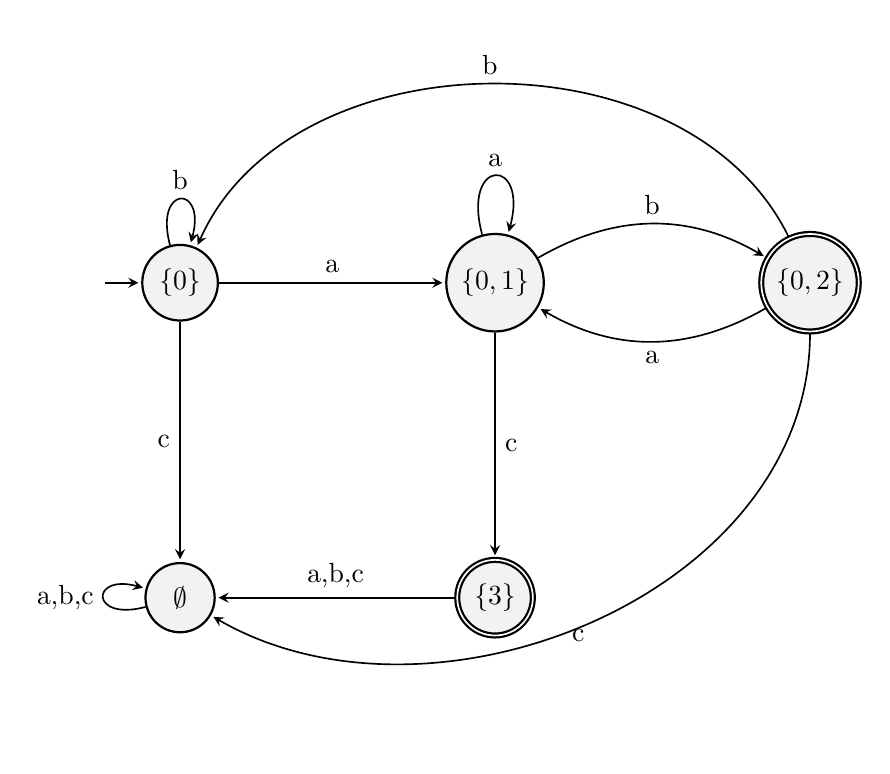
\begin{tikzpicture}[shorten >=1pt, node distance=4cm, on grid, auto, semithick] 
       % States
       \node[state, initial, initial text={}] (q0) {$\{0\}$}; 
       \node[state] (q01) [right=of q0] {$\{0,1\}$}; 
       \node[state, accepting] (q02) [right=of q01] {$\{0,2\}$};
       \node[state, accepting] (q3) [below=of q01] {$\{3\}$};
       \node[state] (empty) [below=of q0] {$\emptyset$};

       \path[->] 
        (q0) edge node {a} (q01)
             edge [loop above] node {b} (q0)
             edge node [left] {c} (empty)
        (q01) edge [loop above] node {a} (q01)
              edge [bend left] node {b} (q02)
              edge node [right] {c} (q3)
        (q02) edge [bend left] node {a} (q01)
              % Single arrow for B going above
              edge [bend right=65] node [above] {b} (q0)
              % Single long arrow for C going below state {3}
              edge [out=270, in=330] node [below left] {c} (empty)
        (q3) edge node [above] {a,b,c} (empty)
        (empty) edge [loop left] node {a,b,c} (empty);
    \end{tikzpicture}
\end{enumerate}

\textbf{Homework 2}

\begin{enumerate}

    \item \textbf{Determinization $\mathcal A^{\mathrm{D}}$ of $\mathcal A$ Transition Table Using the Power Set Construction:}
    
    \vspace{5pt}
    \begin{tabular}{|l|c|c|}
        \hline
        \textbf{States} & \textbf{0} & \textbf{1} \\ \hline
        $\rightarrow \{q_0\}$ & $\{q_0\}$ & $\{q_0, q_1\}$ \\ \hline
        $\{q_0, q_1\}$ & $\{q_0\}$ & $\{q_0, q_1, q_2\}$ \\ \hline
        $\{q_0, q_1, q_2\}$ & $\{q_0, q_1, q_3\}$ & $\{q_0, q_1, q_2\}$ \\ \hline
        $\{q_0, q_1, q_3\}$ & $\{q_0, q_3\}$ & $\{q_0, q_1, q_2, q_3\}$ \\ \hline
        $\{q_0, q_3\}$ & $\{q_0, q_3\}$ & $\{q_0, q_1, q_3\}$ \\ \hline
        $\{q_0, q_1, q_2, q_3\}$ & $\{q_0, q_1, q_3\}$ & $\{q_0, q_1, q_2, q_3\}$ \\ \hline
    \end{tabular}

    \vspace{20pt}
    \textbf{Determinization $\mathcal A^{\mathrm{D}}$ of $\mathcal A$ Diagram Using the Power Set Construction:}


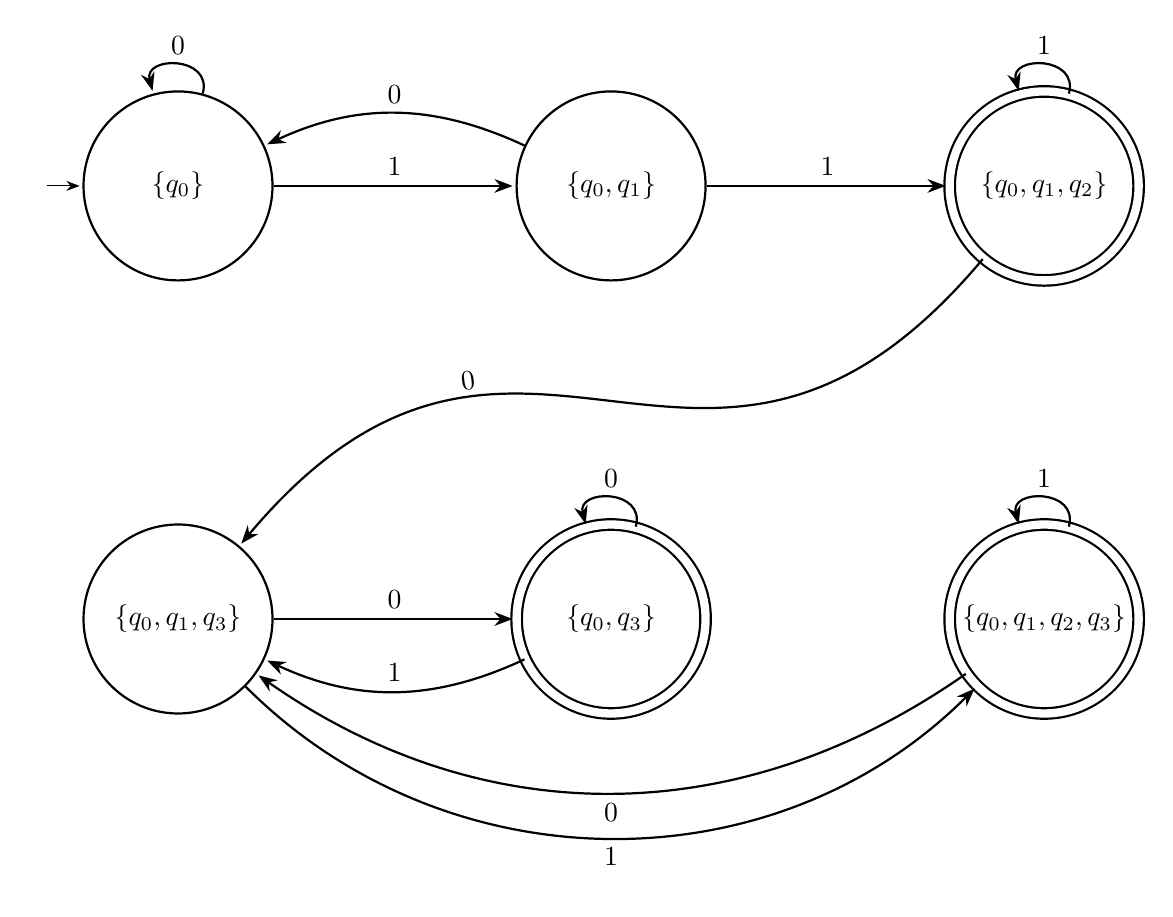
\begin{tikzpicture}[
    shorten >=1pt, 
    node distance=5.5cm, 
    on grid, 
    auto,
    % Increased minimum size slightly for label breathing room
    every state/.style={inner sep=1pt, minimum size=2.4cm, thick},
    % Making the 'accepting' (double circle) very visible
    accepting/.style={double distance=3pt, thick},
    >=Stealth,
    % Looseness=0.4 makes the loops very small and tight
    every loop/.style={looseness=0.4, min distance=5mm, in=105, out=75}
]

    % --- Nodes (States) ---
    % Row 1
    \node[state, initial, initial text=] (q0) {$\{q_0\}$};
    \node[state] (q01) [right=of q0] {$\{q_0, q_1\}$};
    \node[state, accepting] (q012) [right=of q01] {$\{q_0, q_1, q_2\}$};

    % Row 2
    \node[state] (q013) [below=of q0] {$\{q_0, q_1, q_3\}$};
    \node[state, accepting] (q03) [below=of q01] {$\{q_0, q_3\}$};
    \node[state, accepting] (q0123) [below=of q012] {$\{q_0, q_1, q_2, q_3\}$};

    % --- Transitions ---
    \path[->, thick] 
        % State {q0}
        (q0)   edge [loop above] node {0} (q0)
               edge node {1} (q01)
        
        % State {q0, q1}
        (q01)  edge [bend right=25] node [above] {0} (q0)
               edge node {1} (q012)
        
        % State {q0, q1, q2} 
        % Path curves widely to avoid {q0, q1}
        (q012) edge [out=230, in=50, looseness=1.4] node [pos=0.7, sloped, above] {0} (q013)
               edge [loop above] node {1} (q012)
        
        % State {q0, q1, q3}
        (q013) edge node {0} (q03)
               % Bend right 45 ensures it stays well below {q0, q3}
               edge [bend right=45] node [below] {1} (q0123)
        
        % State {q0, q3}
        (q03)  edge [loop above] node {0} (q03)
               edge [bend left=25] node [above] {1} (q013)
        
        % State {q0, q1, q2, q3}
        (q0123) edge [bend left=35] node [below] {0} (q013)
                edge [loop above] node {1} (q0123);

\end{tikzpicture}
     \item There is a smaller DFA where $\{q_0,q_1,q_3\}$, $\{q_0,q_3\}$, $\{q_0,q_1,q_2,q_3\}$ will be merged into one accepting state. This is due to all of them leading back to each other despite the input; they are essentially equivalent.
\end{enumerate}


\subsubsection{Question}
Do you always have to change NFAs to be DFAs when programming?

\subsection{Week 4}

\subsubsection{HW 4}

\textbf{Exercise (Kleene's Algorithm)}

$k=0$:
\begin{align*}
R_{11}^{(0)} &= \varepsilon + a \\
R_{12}^{(0)} &= b \\
R_{21}^{(0)} &= a \\
R_{22}^{(0)} &= \varepsilon + b
\end{align*}

$k=1$:
\begin{align*}
R_{11}^{(1)} &= R_{11}^{(0)} + R_{11}^{(0)}(R_{11}^{(0)})^* R_{11}^{(0)} \\
&= (\varepsilon + a) + (\varepsilon + a)(\varepsilon + a)^* (\varepsilon + a) \\
&= a^* \\[10pt]
%
R_{12}^{(1)} &= R_{12}^{(0)} + R_{11}^{(0)}(R_{11}^{(0)})^* R_{12}^{(0)} \\
&= b + (\varepsilon + a)(\varepsilon + a)^* b \\
&= a^* b \\[10pt]
%
R_{21}^{(1)} &= R_{21}^{(0)} + R_{21}^{(0)}(R_{11}^{(0)})^* R_{11}^{(0)} \\
&= a + a(\varepsilon + a)^* (\varepsilon + a) \\ 
&= aa^* \\[10pt]
%
R_{22}^{(1)} &= R_{22}^{(0)} + R_{21}^{(0)}(R_{11}^{(0)})^* R_{12}^{(0)} \\
&= (\varepsilon + b) + a(\varepsilon + a)^* b \\
&= \varepsilon + b + aa^* b
\end{align*}

$k=2$:
\begin{align*}
R_{11}^{(2)} &= R_{11}^{(1)} + R_{12}^{(1)}(R_{22}^{(1)})^* R_{21}^{(1)} \\
&= a^* + (a^* b)(\varepsilon + b + aa^* b)^* (aa^*) \\
&= a^* + (a^* b)(b + aa^* b)^* (aa^*)
\end{align*}

\vspace{1cm}
\textbf{Final Regular Expression:}
\[ R = a^* + a^* b (b + aa^* b)^* aa^* \]

\textbf{ITALC, Exercise 4.4.2.}

a. The state minimization table:
\begin{tabular}{c|cccccccc}
    & A & B & C & D & E & F & G & H \\ \hline
    B & X &   &   &   &   &   &   &   \\
    C & X & X &   &   &   &   &   &   \\
    D &   & X & X &   &   &   &   &   \\
    E & X &   & X & X &   &   &   &   \\
    F & X & X &   & X & X &   &   &   \\
    G &   & X & X &   & X & X &   &   \\
    H & X &   & X & X &   & X & X &   \\
    I & X & X &   & X & X &   & X & X \\
\end{tabular}

\vspace{2cm}

b. The minimized DFA diagram:
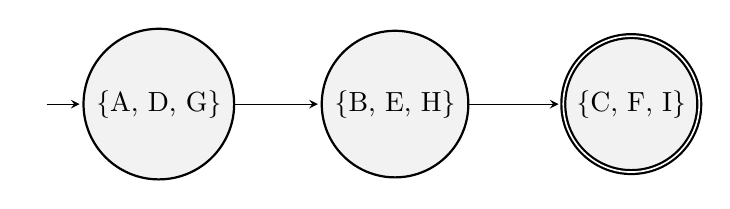
\begin{tikzpicture}[shorten >=1pt, node distance=3cm, on grid, auto]
    \node[state, initial, initial text=] (q0) {\{A, D, G\}};
    \node[state] (q1) [right=of q0] {\{B, E, H\}};
    \node[state, accepting] (q2) [right=of q1] {\{C, F, I\}};

    \path[->] 
        (q0) edge node {} (q1)
        (q1) edge node {} (q2);
\end{tikzpicture}

\subsubsection{Question}
Where would an implementation of Kleene's Algorithm be the most beneficial?

\subsection{Week 5}

\subsubsection{Problems on the Pumping Lemma}

\textbf{Exercise}

\textbf{$L_1 = \{ a^n b^m \in \{a,b\}^* \; | \; n,m \in \mathbb N, ~ n > m \ge 0 \}$}
\begin{itemize}
    \item \textbf{String Choice:} Let $s = a^{p+1}b^p$. Note $s \in L_1$ because $p+1 > p$ and $|s| \ge p$.
    \item \textbf{Decomposition:} $s = xyz$ such that $|xy| \le p$ and $|y| > 0$. Since the first $p$ characters are all $a$'s, $y = a^k$ for some $1 \le k \le p$.
    \item \textbf{Pumping:} Consider $i=0$ (pumping down). The resulting string is $s' = xy^0z = xz$.
    \item \textbf{Contradiction:} The number of $a$'s in $s'$ is $(p+1) - k$. Since $k \ge 1$, $(p+1) - k \le p$. The number of $b$'s remains $p$. Thus, the number of $a$'s is no longer strictly greater than the number of $b$'s ($p-k+1 \not> p$), so $s' \notin L_1$.
\end{itemize}

\textbf{$L_2 = \{ a^{n^2} \in \{a\}^* \; | \; n \in \mathbb N, ~ n \ge 1 \}$}
\begin{itemize}
    \item \textbf{String Choice:} Let $s = a^{p^2}$. Note $s \in L_2$ and $|s| = p^2 \ge p$.
    \item \textbf{Decomposition:} $y = a^k$ where $1 \le k \le p$.
    \item \textbf{Pumping:} Consider $i=2$ (pumping up). The length of $xy^2z$ is $|s| + |y| = p^2 + k$.
    \item \textbf{Contradiction:} We know that $p^2 < p^2 + k$. Since $k \le p$, we also know:
    \[ p^2 + k < p^2 + 2p + 1 = (p+1)^2 \]
    Because $p^2 < |xy^2z| < (p+1)^2$, the length is trapped between two consecutive perfect squares and cannot be a perfect square itself. Thus, $xy^2z \notin L_2$.
\end{itemize}

\textbf{$L_3 = \{ a^p \in \{a\}^\ast \; | \; p \in \mathbb N, ~ p\,\,\mathrm{prime} \}$}
\begin{itemize}
    \item \textbf{String Choice:} Let $n$ be a prime such that $n > p$. Let $s = a^n$.
    \item \textbf{Decomposition:} $y = a^k$ where $1 \le k \le p$. The length of $s$ is $n$.
    \item \textbf{Pumping:} Let $i = n+1$. The length of $xy^{n+1}z$ is:
    \[ |s| + n|y| = n + nk = n(1+k) \]
    \item \textbf{Contradiction:} Since $n > 1$ and $(1+k) > 1$, the length $n(1+k)$ is a composite number. A string of composite length is not in $L_3$, so $L_3$ is not regular.
\end{itemize}

\textbf{$L_4 = \{ a^k b^m a^{k+m} \; | \; k,m \geq 0\}$}
\begin{itemize}
    \item \textbf{String Choice:} Let $s = a^p b^p a^{2p}$. Note $s \in L_4$ because $p + p = 2p$.
    \item \textbf{Decomposition:} Since $|xy| \le p$, $y$ must consist only of $a$'s from the first block. Thus $y = a^j$ for $1 \le j \le p$.
    \item \textbf{Pumping:} Let $i = 2$. The new string is $s' = a^{p+j} b^p a^{2p}$.
    \item \textbf{Contradiction:} For $s' \in L_4$, the sum of the exponents of the first two blocks must equal the exponent of the last block. However, $(p+j) + p = 2p + j$. Since $j \ge 1$, $2p + j \neq 2p$. Thus $s' \notin L_4$.
\end{itemize}

\subsubsection{Question}
Is the pumping lemma specific only to computer science, or could it be applicable to other fields?

\subsection{Week 6}

\subsubsection{HW 6}

\textbf{Turing Machines: Exercise A}

\begin{enumerate}
    \item \textbf{TM for $10^n \to 10^{n+1}$:} 
    \begin{center}
    \begin{tabular}{ccccc}
    \toprule
    State & Read & Write & Move & Next \\ \midrule
    $q_0$ & 1 & 1 & R & $q_1$ \\
    $q_1$ & 0 & 0 & R & $q_1$ \\
    $q_1$ & B & 0 & R & $q_{acc}$ \\ \bottomrule
    \end{tabular}
    \end{center}

    \item \textbf{TM for $10^n \to 1$:} 
    \begin{center}
    \begin{tabular}{ccccc}
    \toprule
    State & Read & Write & Move & Next \\ \midrule
    $q_0$ & 1 & 1 & R & $q_1$ \\
    $q_1$ & 0 & 0 & R & $q_1$ \\
    $q_1$ & B & B & L & $q_2$ \\
    $q_2$ & 0 & B & L & $q_2$ \\
    $q_2$ & 1 & 1 & R & $q_{acc}$ \\ \bottomrule
    \end{tabular}
    \end{center}

    \item \textbf{TM for Swapping 0's and 1's:}
    \begin{center}
    \begin{tabular}{ccccc}
    \toprule
    State & Read & Write & Move & Next \\ \midrule
    $q_0$ & 1 & 0 & R & $q_0$ \\
    $q_0$ & 0 & 1 & R & $q_0$ \\
    $q_0$ & B & B & R & $q_{acc}$ \\ \bottomrule
    \end{tabular}
    \end{center}
\end{enumerate}

\textbf{Problems on Decidability: Exercise 1}
\begin{enumerate}
    \item \textbf{True.} Since $L_1$ and $L_2$ are decidable, there exist TMs $M_1, M_2$ that halt on all inputs. A TM for $L_1 \cup L_2$ runs $M_1$ then $M_2$; it accepts if either accepts and rejects if both reject.
    
    \item \textbf{True.} If $M$ decides $L$, we construct $M'$ to decide $\overline{L}$ by swapping the $q_{accept}$ and $q_{reject}$ states of $M$.
    
    \item \textbf{True.} Decidable languages are closed under Kleene star. We can use a dynamic programming approach to check if any prefix $w[1 \dots i] \in L$ and the remainder $w[i+1 \dots n] \in L^*$.
    
    \item \textbf{True.} To recognize $L_1 \cup L_2$, run TMs $M_1$ and $M_2$ in parallel (interleaving steps). If either halts and accepts, the union TM accepts.
    
    \item \textbf{False.} The language $A_{TM}$ (the Halting Problem) is r.e., but its complement $\overline{A_{TM}}$ is not r.e.
    
    \item \textbf{True.} We can construct a non-deterministic TM that non-deterministically branches to split the input into $k$ substrings and verifies each substring is in $L$.
\end{enumerate}

\subsubsection{Question}
Are there concepts similar to Turing Machines in other fields or are Turing Machines unique to Computer Science?

\subsection{Week 7}

\subsubsection{HW 7}

\textbf{Problems on Decidability: Exercise 2}
\begin{enumerate}
    \item \textbf{$L_1 := \{M \mid M \text{ halts on itself}\}$}
    \begin{itemize}
        \item \textbf{Recursively Enumerable (r.e.): Yes.} We can build a Universal Turing Machine that takes the description of $M$ and simulates $M$ using its own description $\langle M \rangle$ as input. If $M$ halts, the simulation will eventually halt and accept.
        \item \textbf{Decidable: No.} This is proven via a reduction from the standard Halting Problem. If we could decide $L_1$, we could decide if any machine $M$ halts on any input $w$ by constructing a new machine $M'$ that ignores its own input and simply runs $M(w)$.
        \item \textbf{Co-r.e.: No.} If $L_1$ were co-r.e., and since it is already r.e., it would necessarily be decidable (by running both the r.e. and co-r.e. procedures in parallel). Since it is undecidable, it cannot be co-r.e.
    \end{itemize}

    \item \textbf{$L_2 := \{(M, w) \mid M \text{ halts on the word } w\}$}
    \begin{itemize}
        \item \textbf{Recursively Enumerable (r.e.): Yes.} A Universal Turing Machine can simulate $M$ on $w$. If $M$ halts on $w$, the simulator halts and accepts.
        \item \textbf{Decidable: No.} This is the standard Halting Problem ($ATM$ or $HALT_{TM}$). Alan Turing famously proved that no general algorithm exists to decide this for all possible program-input pairs.
        \item \textbf{Co-r.e.: No.} Similar to $L_1$, if $L_2$ were co-r.e., it would be decidable. The complement (detecting if a machine loops forever) is not r.e.
    \end{itemize}

    \item \textbf{$L_3 := \{(M, w, k) \mid M \text{ halts on } w \text{ in at most } k \text{ steps}\}$}
    \begin{itemize}
        \item \textbf{Decidable: Yes.} This is the "bounded" version of the halting problem. Unlike the previous two, it is decidable because the search space is finite.
        \item \textbf{Argument:} To decide $L_3$, simply simulate $M$ on $w$ for exactly $k$ steps:
        \begin{itemize}
            \item If the machine enters a halting state at or before step $k$, \textbf{Accept}.
            \item If the machine has not halted after $k$ steps, \textbf{Reject}.
        \end{itemize}
        \item \textbf{R.e. and Co-r.e.: Yes.} Since every decidable language is both r.e. and co-r.e. by definition, $L_3$ fits into all three categories.
    \end{itemize}
\end{enumerate}

\textbf{Landau Notation: Exercise 2}
\begin{enumerate}
    \item \textbf{Reflexive Property: $f \in \mathcal{O}(f)$} \\
    Proof: Choose $C = 1$ and $n_0 = 1$. For all $n \geq 1$, it is always true that $f(n) \leq 1 \cdot f(n)$. Since the condition holds, $f \in \mathcal{O}(f)$.

    \item \textbf{Constant Multiples: If $c > 0$ is a constant, then $\mathcal{O}(c \cdot f) = \mathcal{O}(f)$} \\
    We must show both inclusions:
    \begin{itemize}
        \item ($\subseteq$): Let $g \in \mathcal{O}(c \cdot f)$. Then $g(n) \leq C \cdot (c \cdot f(n))$ for $n \geq n_0$. By setting a new constant $C' = C \cdot c$, we get $g(n) \leq C' \cdot f(n)$, so $g \in \mathcal{O}(f)$.
        \item ($\supseteq$): Let $g \in \mathcal{O}(f)$. Then $g(n) \leq C \cdot f(n)$ for $n \geq n_0$. We can rewrite this as $g(n) \leq \frac{C}{c} \cdot (c \cdot f(n))$. Since $c > 0$, $\frac{C}{c}$ is a valid constant, so $g \in \mathcal{O}(c \cdot f)$.
    \end{itemize}

    \item \textbf{Dominance: If $f \leq g$ for large enough inputs, then $\mathcal{O}(f) \subseteq \mathcal{O}(g)$} \\
    Proof: Let $h \in \mathcal{O}(f)$. This means $h(n) \leq C \cdot f(n)$ for $n \geq n_1$. 
    We are given $f(n) \leq g(n)$ for $n \geq n_2$. 
    For all $n \geq \max(n_1, n_2)$, we have $h(n) \leq C \cdot f(n) \leq C \cdot g(n)$. 
    Thus, $h \in \mathcal{O}(g)$.

    \item \textbf{Additive Property: If $\mathcal{O}(f) \subseteq \mathcal{O}(g)$, then $\mathcal{O}(f + h) \subseteq \mathcal{O}(g + h)$} \\
    Proof: The premise $\mathcal{O}(f) \subseteq \mathcal{O}(g)$ implies $f \in \mathcal{O}(g)$, so $f(n) \leq C \cdot g(n)$ for $n \geq n_0$. 
    Take any $t \in \mathcal{O}(f + h)$. Then $t(n) \leq C_1(f(n) + h(n))$ for $n \geq n_1$. 
    Substitute the inequality for $f$: $t(n) \leq C_1(C \cdot g(n) + h(n))$. 
    Let $C_2 = \max(C, 1)$. Then $t(n) \leq C_1 \cdot C_2(g(n) + h(n))$. 
    Since $t$ is bounded by a constant times $(g+h)$, $t \in \mathcal{O}(g + h)$.

    \item \textbf{Multiplicative Property: If $h(n) > 0$ and $\mathcal{O}(f) \subseteq \mathcal{O}(g)$, then $\mathcal{O}(f \cdot h) \subseteq \mathcal{O}(g \cdot h)$} \\
    Proof: From the premise, $f(n) \leq C \cdot g(n)$ for $n \geq n_0$. 
    Let $t \in \mathcal{O}(f \cdot h)$, meaning $t(n) \leq C_1(f(n) \cdot h(n))$ for $n \geq n_1$. 
    Multiply the first inequality by $h(n)$. Since $h(n) > 0$, the direction of the inequality remains the same: $f(n) \cdot h(n) \leq C \cdot g(n) \cdot h(n)$. 
    Therefore, $t(n) \leq C_1(C \cdot g(n) \cdot h(n))$. 
    Using the new constant $C_2 = C_1 \cdot C$, we find $t \in \mathcal{O}(g \cdot h)$.
\end{enumerate}

\subsubsection{Question}
How can we apply Big O algorithms to DFAs, if possible?

\subsection{Week 8}

\subsubsection{Propositional Logic and SAT} 

\textbf{Exercise 1}
\begin{enumerate}
    \item \textbf{Formula $\varphi_1$:}
    \[ \varphi_1 := \neg((a \wedge b) \vee (\neg c \wedge d)) \]
    \textit{Conversion:}
    \begin{align*}
        \varphi_1 &\equiv \neg(a \wedge b) \wedge \neg(\neg c \wedge d) \tag{De Morgan's} \\
        &\equiv (\neg a \vee \neg b) \wedge (c \vee \neg d) \tag{CNF Result}
    \end{align*}

    \item \textbf{Formula $\varphi_2$:}
    \[ \varphi_2 := \neg((p \vee q) \rightarrow (r \wedge \neg s)) \]
    \textit{Conversion:}
    \begin{align*}
        \varphi_2 &\equiv \neg(\neg(p \vee q) \vee (r \wedge \neg s)) \tag{Implication Rule} \\
        &\equiv \neg(\neg(p \vee q)) \wedge \neg(r \wedge \neg s) \tag{De Morgan's} \\
        &\equiv (p \vee q) \wedge (\neg r \vee s) \tag{CNF Result}
    \end{align*}
\end{enumerate}

\textbf{Exercise 2}
\begin{enumerate}
    \item \textbf{$\psi_1 := (a \vee \neg b) \wedge (\neg a \vee b) \wedge (\neg a \vee \neg b)$} \\
    \textbf{Status:} Satisfiable \\
    \textbf{Assignment:} $\{a = \text{False}, b = \text{False}\}$

    \item \textbf{$\psi_2 := (\neg p \vee q) \wedge (\neg q \vee r) \wedge \neg(\neg p \vee r)$} \\
    \textbf{Status:} Unsatisfiable \\
    \textbf{Explanation:} The requirements contradict each other. $p$ makes it so $q$ has to be true, but by $q$ being true, the second clause fails because $r$ must be false.

    \item \textbf{$\psi_3 := (x \vee y) \wedge (\neg x \vee y) \wedge (x \vee \neg y) \wedge (\neg x \vee \neg y)$} \\
    \textbf{Status:} Unsatisfiable \\
    \textbf{Explanation:} The formula represents all four possible combinations of these two variables, $x$ and $y$. The second two clauses have the exact opposite requirements of the first two clauses.
\end{enumerate}

\subsubsection{Question}
Where would propositional logic and SAT be implemented so that it is helpful in simplifying a more complex topic?

\subsection{Week 9}

\subsubsection{Homework: Resolution and Horn Resolution}

\textbf{Exercise 1}

\textbf{1a.}
$\varphi := (a \vee b) \wedge (\neg a \vee c) \wedge (\neg b \vee c) \wedge (\neg c \vee d) \wedge \neg d$

\begin{center}
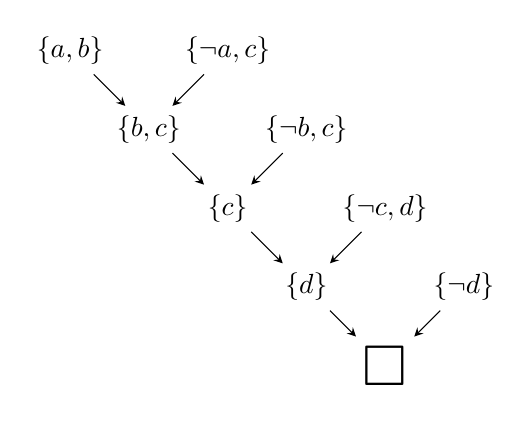
\begin{tikzpicture}[node distance=1.5cm]
  \node (n1) at (0,0) {$\{a, b\}$};
  \node (n2) at (2,0) {$\{\neg a, c\}$};
  \node (n6) at (1,-1) {$\{b, c\}$};
  \draw (n1) -- (n6);
  \draw (n2) -- (n6);

  \node (n3) at (3,-1) {$\{\neg b, c\}$};
  \node (n7) at (2,-2) {$\{c\}$};
  \draw (n6) -- (n7);
  \draw (n3) -- (n7);

  \node (n4) at (4,-2) {$\{\neg c, d\}$};
  \node (n8) at (3,-3) {$\{d\}$};
  \draw (n7) -- (n8);
  \draw (n4) -- (n8);

  \node (n5) at (5,-3) {$\{\neg d\}$};
  \node (n9) at (4,-4) {\huge $\square$};
  \draw (n8) -- (n9);
  \draw (n5) -- (n9);
\end{tikzpicture}
\end{center}

$\varphi$ is unsatisfiable.

\hrule
\vspace{1cm}

$\psi := p \wedge q \wedge (\neg p \vee \neg q \vee r) \wedge (\neg r \vee s) \wedge \neg s$

1. This is a Horn Formula because the clauses can be categorized into three main types based on their structure:
\begin{itemize}
    \item \textbf{Definite Clauses:} contain only one positive literal.
    \item \textbf{Facts:} a special case of definite clauses where there are no negative literals, forcing a variable to be true.
    \item \textbf{Goal Clauses:} contain no positive literals, representing constraints or queries to be disproven.
\end{itemize}

2. \textbf{Resolution Diagram:}
\begin{center}
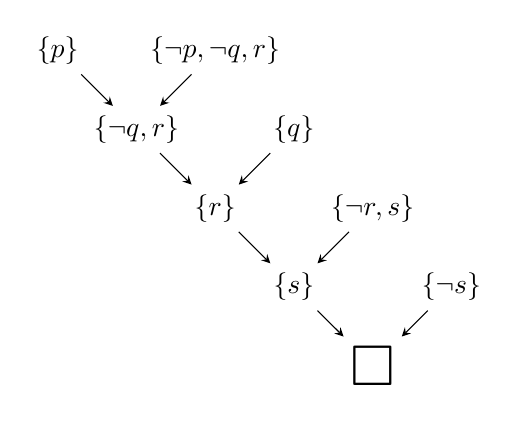
\begin{tikzpicture}[node distance=1.5cm]
  \node (p1) at (0,0) {$\{p\}$};
  \node (p2) at (2,0) {$\{\neg p, \neg q, r\}$};
  \node (p6) at (1,-1) {$\{\neg q, r\}$};
  \draw (p1) -- (p6);
  \draw (p2) -- (p6);

  \node (p3) at (3,-1) {$\{q\}$};
  \node (p7) at (2,-2) {$\{r\}$};
  \draw (p6) -- (p7);
  \draw (p3) -- (p7);

  \node (p4) at (4,-2) {$\{\neg r, s\}$};
  \node (p8) at (3,-3) {$\{s\}$};
  \draw (p7) -- (p8);
  \draw (p4) -- (p8);

  \node (p5) at (5,-3) {$\{\neg s\}$};
  \node (p9) at (4,-4) {\huge $\square$};
  \draw (p8) -- (p9);
  \draw (p5) -- (p9);
\end{tikzpicture}
\end{center}

3. $\psi$ is unsatisfiable.

\textbf{Exercise 2}

\textbf{1. Formalization}
\textbf{Propositional Variables:}
\begin{itemize}
    \item $GPS$: GPS lock is valid.
    \item $BH$: Battery health is good.
    \item $MOK$: Manual override key is present.
    \item $MP$: Motor power is enabled.
\end{itemize}

\textbf{Controller Policy ($\Phi$):}
\begin{enumerate}
    \item $(GPS \wedge BH) \rightarrow MP \equiv (\neg GPS \vee \neg BH \vee MP)$ 
    \item $MOK \rightarrow MP \equiv (\neg MOK \vee MP)$ 
    \item $\neg BH \rightarrow \neg MP \equiv (BH \vee \neg MP)$ 
\end{enumerate}

\textbf{Incident Log Reports ($\gamma$):}
Based on the log (GPS valid, battery unhealthy, manual override present, motor power enabled):
\[ \gamma := GPS \wedge \neg BH \wedge MOK \wedge MP \] 

\textbf{2. Set of Clauses}
The combined knowledge base $\Phi \wedge \gamma$ results in the following clauses:
\[ \mathcal{C} = \{ \{\neg GPS, \neg BH, MP\}, \{\neg MOK, MP\}, \{BH, \neg MP\}, \{GPS\}, \{\neg BH\}, \{MOK\}, \{MP\} \} \] 

\textbf{3. Consistency Analysis}
    \begin{forest}
    for tree={
        math content, 
        grow=north,   
        edge={-},
        l sep=1.5em,
        s sep=2em
    }
    [ {\square} 
        [ {\{\neg MP\}} 
            [ {\{BH, \neg MP\}}, tier=top ] 
            [ {\{\neg BH\}}, tier=top ]
        ]
        [ {\{MP\}} 
            [ {\{MP\}}, tier=top, no edge ] % This removes the line
        ] 
    ]
\end{forest}

\textbf{Conclusion:} 
Because the empty clause $\square$ is derived, the Log is \textbf{inconsistent} with the Policy.

\textbf{4. Conflict Identification}
The policy dictates that if battery health is bad ($\neg BH$), motor power must be blocked ($\neg MP$). However, the log reports the motor power was enabled ($MP$). This occurred because the manual override key ($MOK$) was used, which allowed power despite the battery safety interlock.

\subsubsection{Question}
Can we use resolution or Horn's resolution in any aspects of turing machines?

\section{Synthesis}

\section{Evidence of Participation}

\section{Conclusion}\label{conclusion}

\begin{thebibliography}{99}
\bibitem[BLA]{bla} Author, \href{https://en.wikipedia.org/wiki/LaTeX}{Title}, Publisher, Year.
\end{thebibliography}

\end{document}
